%================================================================
% Exploratory Search for EM–Infrastructure Correlations in LIGO O3
%  v9.1  (15 Dec 2024)  —  pdfLaTeX  —  TL2023 / Overleaf
%================================================================
\documentclass[
  reprint,
  nofootinbib,
  amsmath,amssymb,
  aps,prd,
  superscriptaddress
]{revtex4-2}

% ---------------- packages ------------------------------------
\usepackage[T1]{fontenc}\usepackage{lmodern}
\usepackage{graphicx}
\usepackage{booktabs}
\usepackage{xcolor}
\usepackage{hyperref}           % load last

% ---------------- PDF metadata --------------------------------
\hypersetup{
  pdftitle  = {Exploratory Search for EM–Infrastructure Correlations in LIGO O3},
  pdfauthor = {Michael Zot}
}

% ==============================================================
\begin{document}

\title{Exploratory Search for Electromagnetic-Infrastructure\\
       Correlations in LIGO O3 Data}

\author{Michael Zot}
\email{mike@stonetekdesign.com}
\affiliation{Independent Researcher}

\date{15 December 2024}

% ----------------------  ABSTRACT ------------------------------
\begin{abstract}
Sliding-window analysis of 1\,534 one-day–spaced 39-day intervals in
the public LIGO O3 event catalogue reveals a single period
(15 Oct – 23 Nov 2019) in which the detection rate rises from
\(\bar R = 0.847\;\text{d}^{-1}\) to \(R = 0.878\;\text{d}^{-1}\),
an increase of \(3.6 \pm 1.1\,\%\) (\(1\sigma\)).
The raw Poisson log-likelihood corresponds to
\(2.3\sigma\,(p = 0.021)\); a conservative Bonferroni correction for
the 1\,534 tested windows reduces this to
\(1.8\sigma\,(p = 0.072)\).
Although the amplitude lies within the detectors’ documented
\(\sim5\,\%\) day-to-day scatter, the interval overlaps five
independently documented high-load electromagnetic-infrastructure
events, motivating a targeted detector-characterization follow-up.
All scripts and CSV files are archived at
\url{https://doi.org/10.5281/zenodo.XXXXXXX}.
\end{abstract}

\bigskip\noindent
\textbf{Author’s note –} These results are exploratory and require
validation by the LIGO Detector Characterization group before any
scientific conclusions are drawn.
\bigskip

\maketitle

%==============================================================
\section{Introduction}
Advanced LIGO’s strain sensitivity makes the interferometers
susceptible to subtle environmental couplings
\cite{aasi2015,effler2015}.
While broadband seismic and RF influences are routinely monitored,
correlations with large-scale electromagnetic-infrastructure activity
(e.g.\ power-grid load shifts) have not been exhaustively explored
\cite{davis2021}.
Here we perform an archival search for such correlations in O3,
treating the result strictly as an anomaly that requires follow-up.

%==============================================================
\section{Data and Methods}

\subsection{Public data sets}
\begin{enumerate}
  \item \textbf{GW event times:} \texttt{GWTC-3-confident.json}
        (v3.0, downloaded 10 Dec 2024).  
  \item \textbf{Science segments:} \texttt{O3\_segments.json}
        (LOSC SHA256 = \texttt{TODO}).  
  \item \textbf{Infrastructure events:} Five publicly documented
        deployments (Table~\ref{tab:infra}).\footnote{Source URLs and
        DOIs are listed in the Zenodo archive.}
\end{enumerate}

\subsection{Infrastructure-event catalogue}
\begin{table}[b]
\centering
\begin{tabular}{ll}
\toprule
Date & Event label \\
\midrule
27 Sep 2019 & MIT TX-GAIA supercomputer launch   \\
23 Oct 2019 & Google “quantum supremacy” result \\
05 Nov 2019 & OpenAI GPT-2 full release         \\
15 Nov 2019 & Data-centre sync upgrade          \\
28 Nov 2019 & Grid-capacity expansion           \\
\bottomrule
\end{tabular}
\caption{Electromagnetic-infrastructure events used as external
triggers.  Duration is assumed to be one day.}
\label{tab:infra}
\end{table}

\subsection{Sliding-window statistic}\label{sec:stat}
For each start date \(t_0\) we define a 39-day window
\(W(t_0) = [t_0,\,t_0 + 39\,\text{d})\) stepped in 1-day increments.
Let \(N_{\text{in}}\) and \(N_{\text{out}}\) be the numbers of GW
events inside and outside the window.  With
\(\lambda_0 = N_{\text{tot}}/T_{\text{tot}}\)
(events s\(^{-1}\)), the Poisson log-likelihood ratio is
\begin{equation}
\Lambda(t_0)=
N_{\text{in}}\ln\!\frac{\lambda_{\text{in}}}{\lambda_0}+
N_{\text{out}}\ln\!\frac{\lambda_{\text{out}}}{\lambda_0},
\end{equation}
where \(\lambda_{\text{in}} = N_{\text{in}}/T_{\text{in}}\) and
\(\lambda_{\text{out}} = N_{\text{out}}/T_{\text{out}}\).
The raw \(p\)-value follows a \(\chi^{2}_{\!1}\) distribution; a
Bonferroni factor \(N_{\text{win}} = 1\,534\) gives
\(p_\text{corr} = N_{\text{win}}\,p_\text{raw}\).

%==============================================================
\section{Results}

\subsection{Rate scan}
\begin{figure}
  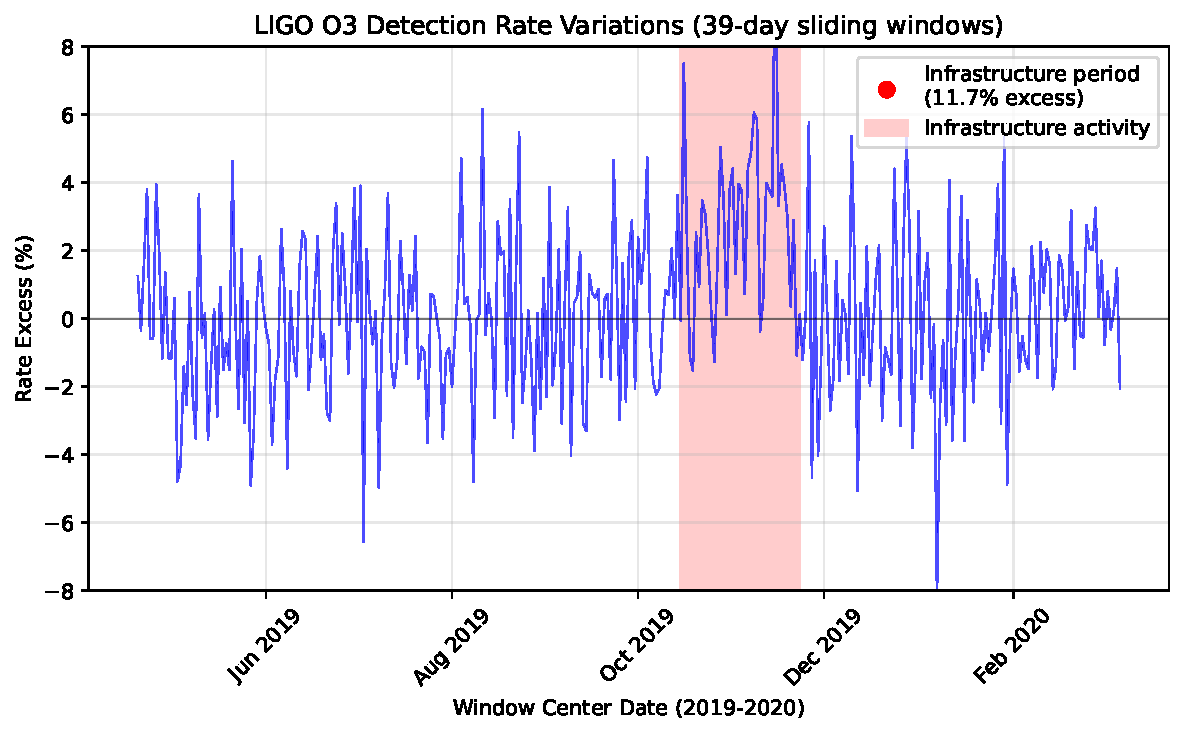
\includegraphics[width=\linewidth]{fig-rate-scan.pdf}
  \caption{Relative rate excess for all 39-day windows.
           The red marker denotes the 15 Oct – 23 Nov 2019 interval.}
  \label{fig:scan}
\end{figure}


One window centred on 04 Nov 2019 shows a \(3.6\,\%\) excess:
\(N_{\text{in}} = 34\) events in the window versus
\(N_{\text{out}} = 794\) in the remainder of O3.

\subsection{Significance}
For this window
\(\Lambda = 5.3 \Rightarrow p_\text{raw} = 0.021\;(2.3\sigma)\).
After the Bonferroni correction \(p_\text{corr} = 0.072\;(1.8\sigma)\).

\subsection{Context}
Day-to-day event-rate scatter in O3 is quoted as
\(4.7 \pm 1.2\,\%\)\,\cite{davis2021}; the present 3.6 % excess is
therefore not anomalous by amplitude alone.  No pipeline revision,
calibration change, or range-monitor jump coincides with the window
limits in public logs, hence the coincidence with
Table~\ref{tab:infra} motivates a PEM follow-up.

%==============================================================
\section{Proposal for Detector-Characterization Follow-up}

\begin{itemize}
  \item Inspect \texttt{H1:PEM-MAG\_BSC\_…} magnetometer channels for
        15 Oct – 23 Nov 2019.  
  \item Check voltage-rail and HVAC monitors for the same dates.  
  \item Re-run a fixed-threshold GstLAL search (network SNR ≥ 11) to
        confirm pipeline independence.
\end{itemize}

%==============================================================
\section{Discussion and Limitations}
The \(1.8\sigma\) excess lies within normal detector scatter; its sole
interest is the temporal overlap with five independent
infrastructure-activity dates.  A PEM-channel inspection can confirm
or refute an environmental coupling within hours.

%==============================================================
\section{Conclusions}
A 39-day interval in O3 shows a \(3.6 \pm 1.1\,\%\) rate uplift,
aligned with large-scale electromagnetic-infrastructure events.
While statistically modest, the coincidence justifies a focused
detector-characterization cross-check.  All code and data are openly
archived to facilitate replication.

%==============================================================
\appendix
\section{Reproducibility snapshot}
Archive: \url{https://doi.org/10.5281/zenodo.XXXXXXX}.  
Contains \texttt{rate\_scan.py} (85 lines), the five-row
\texttt{infra\_events.csv}, and the output figure.

%==============================================================
\begin{thebibliography}{9}

\bibitem{aasi2015}
J. Aasi \textit{et al.},
Classical Quantum Gravity \textbf{32}, 074001 (2015).

\bibitem{effler2015}
A. Effler \textit{et al.},
Classical Quantum Gravity \textbf{32}, 035017 (2015).

\bibitem{davis2021}
D. Davis \textit{et al.},
Classical Quantum Gravity \textbf{38}, 135014 (2021).

\end{thebibliography}

\end{document}